% FACULTAD DE INGENIERÍA, UNIVERSIDAD DE BUENOS AIRES
%
% 75.10 - Técnicas de Diseño
% Trabajo práctico nro 2
%
% INFORME

\documentclass[12pt]{article}

\usepackage[a4paper,headheight=16pt,scale={0.7,0.8},hoffset=0.5cm]{geometry}
\usepackage[spanish]{babel}
\usepackage{graphicx}
\usepackage[utf8]{inputenc}

% Para poner el texto "Figura X" en negrita:
\usepackage[hang,bf]{caption}

% Símbolos varios.
\usepackage{textcomp}

\title{Técnicas de Diseño: TP2}
\author{Barrios, Federico; Bosch, Florencia; Navarro, Patricio}

%------------------------- Inicio del documento ---------------------------
\begin{document}

\begin{center}
\vspace*{7 cm}
\textsc{\LARGE Universidad de Buenos Aires}\\[0.3cm]
\textsc{\LARGE Facultad de Ingeniería}\\[1.2cm]
\textsc{\Large 75.10 -- Técnicas de Diseño}\\[0.3cm]
\textsc{\Large Trabajo Práctico 2}\\[1.2cm]
\end{center}

\begin{flushright}
{\large
Grupo 3:\\[0.1cm]
Barrios, Federico -- 91954\\
Bosch, Florencia -- 91867\\
Navarro, Patricio -- 90007\\[0.4cm]
$2^{do}$ cuatrimestre de 2013}
\end{flushright}

\thispagestyle{empty}

\newpage

% Pongo el índice en una página aparte:
\tableofcontents
% Hago que las páginas se comiencen a contar a partir de aquí:
\setcounter{page}{1}
\newpage

\section{Especificación}
Se propone implementar un framework de testing unitario que provea diferentes
tipos de aserciones y que finalmente genere un reporte de resultados.

Entre las restricciones se encuentra el no poder usar reflexión para identificar
y ejecutar los métodos, sino que se debe implementar mediante un modelo de 
dominio.


\section{Análisis}
Se debe proveer al usuario un entorno para desarrollar pruebas unitarias, por lo
que se le deberá proveer al usuario una serie de métodos para realizar 
verificaciones sobre instancias de sus clases. Se decició poner a disposición 
del usuario un subconjunto reducido de las aserciones que brinda jUnit 4:\footnote{
La lista completa de aserciones de jUnit 4 está disponible en: \\
http://junit.sourceforge.net/javadoc/org/junit/Assert.html}
	\begin{itemize}
		\item \textbf{fail}: esta verificación siempre falla, suele usarse para
			mostrar que hay métodos que no están implementados
			en su totalidad.
		\item \textbf{assertTrue} y \textbf{assertFalse}: ambas aserciones toman un 
			objeto como parámetro y verifican que sea verdadero ó 
			falso respectivamente.
		\item \textbf{assertEquals} y \textbf{assertNotEquals}: ambas aserciones toman dos
			objetos como parámetros y verifican que sean iguales ó 
			diferentes respectivamente; teniendo en cuenta el método
			equals() de la clase a probar.
		\item \textbf{assertSame} y \textbf{assertNotSame}: ambas aserciones toman dos 
			objetos como parámetros y verifican que sean la misma 
			o diferente instancia de la clase respectivamente; 
			comparando sus referencias.
		\item \textbf{assertNull} y \textbf{assertNotNull}: ambas aserciones toman un 
			objeto como parámetro y verifican que se trate de una
			referencia nula o no, respectivamente.
	\end{itemize}
	
Para la segunda parte del trabajo se especificó agregar un set de funcionalidades tales como
ejecución de tests de acuerdo a una expresión regular, implementación de un fixture y permitir
la carga de test suites en niveles ilimitados.
	
\section{Diseño}
El grupo decidió usar el patrón de diseño composite dado que nos brinda la 
posibilidad de agrupar clases que contengan a otras clases y que todas compartan
métodos. De esta manera se permitió que conjuntos de pruebas (test suites) 
contengan casos de pruebas (test cases).

Así se implementaron las clases troncales del trabajo: BaseTest representa la 
hoja (leaf) del patrón composite y es la clase abstracta de la que el usuario 
heredará para correr las pruebas. TestSuite es una clase concreta que toma el 
rol de composite en el patrón, y que contiene instancias de objetos que 
implementen la interfaz RunnableTest, el componente en el patrón.

Los resultados de las pruebas se almacenan en una clase llamada TestResult,
mientras que existe otra clase llamada TestOutput encargada de imprimir esos
resultados, garantizando un desacoplamiento total entre las partes.

El cliente de la estructura composite es una clase llamada TestRunner que
simplemente instancia una nueva clase TestResult y la pasa por parámetro para 
que se almacene allí la información de la corrida.

\begin{figure}[h!]
\begin{center}
	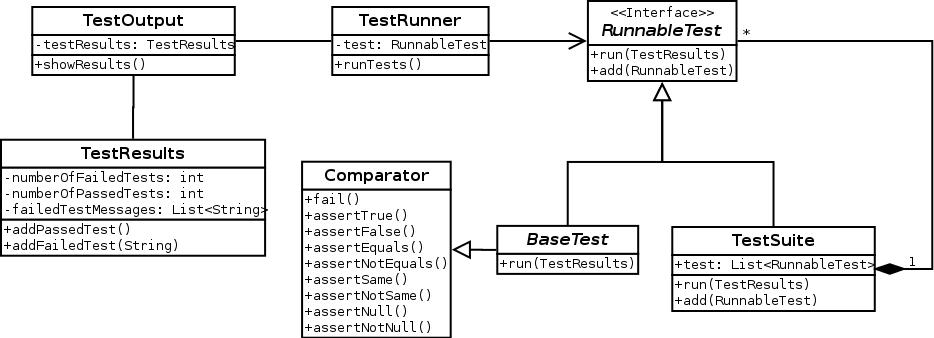
\includegraphics[scale=0.50,angle=90]{./ClassDiagram}
\end{center}
	\caption{diagrama de clases del trabajo práctico (entrega 1).}
\end{figure}

Finalmente existe una clase Comparator que es la encargada de implementar las 
aserciones.

Se muestra toda la estructura de la primera parte de la entrega en la figura 1.

\subsection{Segunda entrega}
Para la segunda entrega se hizo uso del patrón de diseño Template Method para 
implementar la funcionalidad de fixture de testing. Se conservó la estructura
de árbol con el patrón Composite para garantizar la jerarquía de suites y cases
ilimitada.

Se utilizó además el patrón Prototype para clonar instancias de los setUps, de
manera que los test cases no modifiquen la información de los fixtures.
Se implementó la clase TestContext para agrupar estas funcionalidades; que a su
vez está contenida en una llamada TestInformation, que aloja el resultado de los
tests corridos, la salida, y la expresión regular a aplicar, usando una estrategia
de tipo Parameter Object.

Pudimos comprobar que el diseño anterior estuvo abierto a modificaciones, dado que
las funcionalidades requeridas en esta segunda parte fueron agregadas casi sin
hacer mayores modificaciones a la estructura anterior.

Para esta entrega se implementó el diagrama de clases mostrado en la figura 2.

\begin{figure}[h!]
\begin{center}
	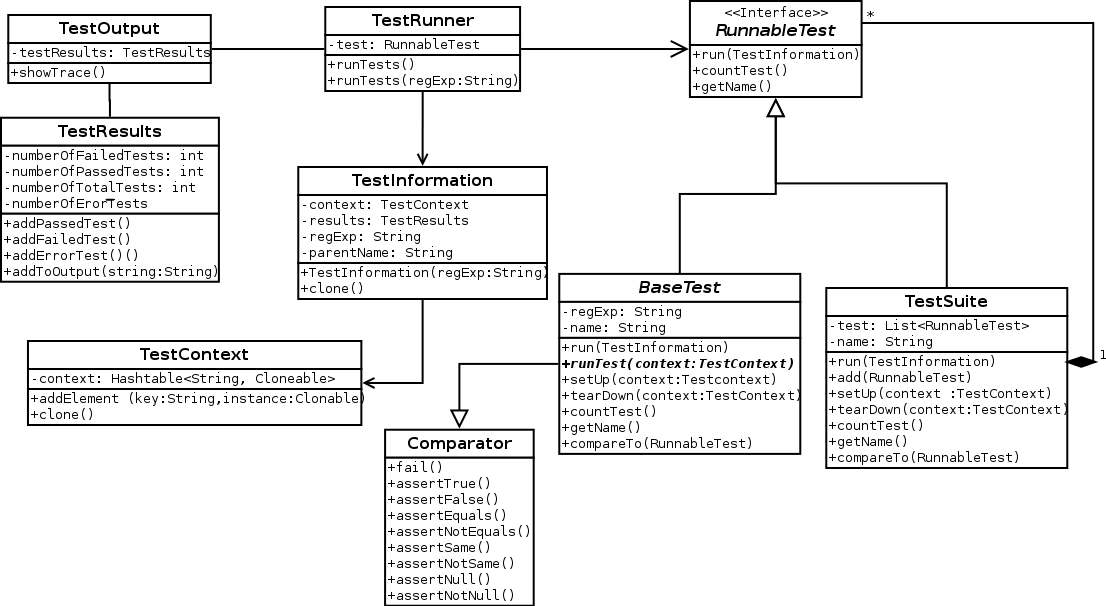
\includegraphics[scale=0.50,angle=90]{./ClassDiagram2}
\end{center}
	\caption{diagrama de clases del trabajo práctico (entrega 2).}
\end{figure}


\subsection{Responsabilidades de las clases}
Se describe a continuación la responsabilidad de cada clase:
\begin{itemize}
	\item \textbf{BaseTest}: es la encargada de correr cada test unitario.
		Las clases que hereden de ella implementarán el código que 
		ejecuta las pruebas. 
		
	\item \textbf{Comparator}: es la clase que implementa las aserciones.	
	
	\item \textbf{TestOutput}: es la encargada de interpretar los resultados
		y producir una salida legible.		
			
	\item \textbf{TestResults}: es una clase almacenadora de información
		sobre la ejecución de las pruebas.
	
	\item \textbf{TestSuite}: es la clase contenedora de todos los tests.
		Permite agregar tests y correrlos.
		
	\item \textbf{TestRunner}: es el cliente en el esquema composite, crea
		una instancia de TestResults, ejecuta un TestSuite y luego
		muestra los resultados usando un TestOutput.	
		
	\item \textbf{TextInformation}: es una clase nueva introducida para 
		encapsular la información de los test corridos anteriormente
	
	\item \textbf{TestContext}: esta clase contiene las instancias creadas
		por los usuarios a la hora de hacer setUps, y es utilizada
		a lo largo de toda la ejecución.

\end{itemize}

\section{Pruebas}
Se incluyen con la implementación varios sets de pruebas:

	\begin{enumerate}
	\item Pruebas unitarias: estas pruebas verifican el funcionamiento de 
	las clases desarrolladas usando jUnit 4. 
	
	Se intentó alcanzar una cobertura del 100\% del código con pruebas 
	unitarias, sin embargo se notó que había varias clases muy simples como 
	TestResult que probarlas pareció inútil.

	\item Pruebas de entorno: la intención de estas pruebas fue probar una 
	clase externa como lo haría el usuario.
	Se creo una clase con un comportamiento trivial y se generaron casos de
	prueba para después correrlos. 
	
	Se insertaron tanto pruebas que corren correctamente como pruebas que
	fallan, de manera de mostrar el funcionamiento completo del entorno.
	
	El mismo de set de pruebas se corrió con jUnit 4 para mostrar que 
	efectivamente los resultados obtenidos son equivalentes.
		\begin{enumerate}
		\item Pruebas de comparación: que verifican que funcione 
		correctamente las aserciones del framework ante diferentes 
		situaciones.
		\item Pruebas de anidación: que verifican que se ejecuten todos
		los casos de prueba en una corrida, anidando varios niveles
		de suites con casos.
		\item Pruebas de expresiones regulares: que verifican que se
		respete que sólo se corran aquéllas pruebas que cumplan con
		la expresión regular indicada.
		\item Pruebas de fixture: que verifican que se respeten los setUps
		y los tearDowns que corresponden para cada corrida.
		\end{enumerate}
	\end{enumerate}

\end{document}
